\chapter{Background}
\label{cha:bg}

This chapter will cover some of the background material required for the following sections, it will cover the history of reinforcement learning (RL) and the fields evolution to the current state-of-the-art. Additionally, it will cover the related work to this project and also cover some details of the past research papers for which this project has been based upon.

\section{Reinforcement learning}
\label{bg:sec:rl}
Reinforcement learning is an area of machine learning has has been under active research since the late 1980s \cite{watkins-phd}. The first defining algorithm of RL was called \textit{`temporal-difference learning'} often referred to as TD-Learning. This algorithm learns by bootstrapping from the current value function in order iteratively converge towards a optimal policy (i.e. the agent's strategy for taking actions in the environment).

Further work by R. Sutton led to the development of TD-Lambda, an algorithm that was applied to the game of Backgammon, in 1992, by Gerald Tesauro to create TD-Gammon \cite{td-gammon}. It was a computer program that was shown to compete at expert-human level. The program also found novel strategies that were either unexplored, or dismissed in error as poor strategies. This was the first example of RL aiding in discovery or reconsideration of board game strategies. This trend of RL algorithms helping to improve human play would prove to only continue with DeepMind's AlphaZero program mastering the games of Chess (beating the strongest Chess programs such as Stockfish\footnote{\href{https://stockfishchess.org}{Stockfish}. One of the strongest Chess programs based on the CCRL ratings list.}) and Go.

\subsection{Deep reinforcement learning}
\label{bg:sec:deeprl}
Following from section \ref{bg:sec:rl} on RL, this section talks about the combination of two areas, deep learning and reinforcement learning methods, called deep reinforcement learning (DRL). Deep learning (DL) is a common class of machine learning methods that has been of much research focus over the past decade and can deal with high-dimensional sensory input; for the case of Atari this is 84x84 greyscale images after pre-processing of the raw Atari frames. On the other hand, reinforcement learning allows us to create an agent which can learn an optimal policy to navigate some environment in order to optimise its reward.

\begin{figure}[htbp]
	\centering
	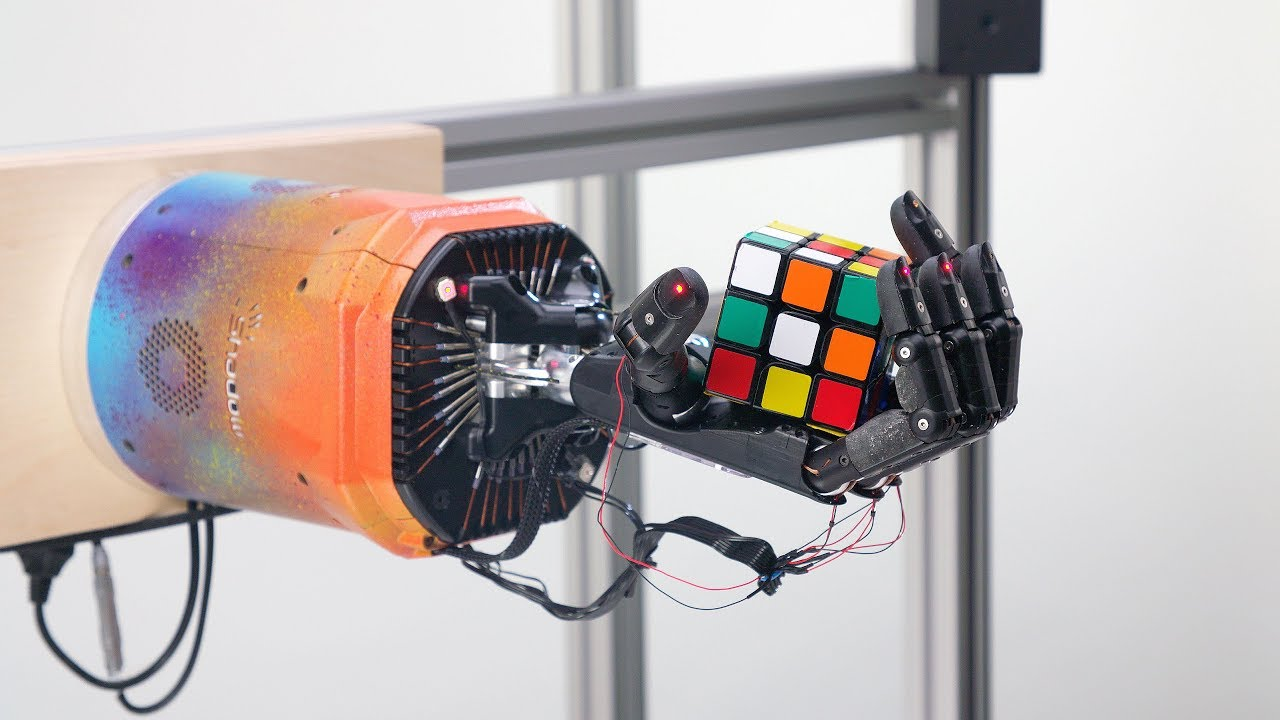
\includegraphics[width=0.5\textwidth]{chapters/chapter2/images/openai-robot.jpg}
	\caption{OpenAI Robot solving a Rubik's cube
		\label{fig:openai-robot}
	}
\end{figure}

Through the combination of these methods, it has proven to provide solutions to previously intractable problems \cite{rl-survey} in areas such as robotics, computer vision and healthcare. For example, in 2019 OpenAI developed a robotic hand that could solve a Rubik's cube \ref{fig:openai-robot}, trained using deep reinforcement learning. As an extension to DRL, end-to-end reinforcement learning is a method for single layered neural network, trained by reinforcement learning. Figure \ref{fig:e2e-rl} shows, diagramatically, how DL and RL are used together in order to produce a single end-to-end model. In this simple architcture, there are two main components, the agent and the environment. This is a key feature of all DRL methods, an agent observes some state and reward from the environment after taking an action.

\begin{figure}[htbp]
	\centering
	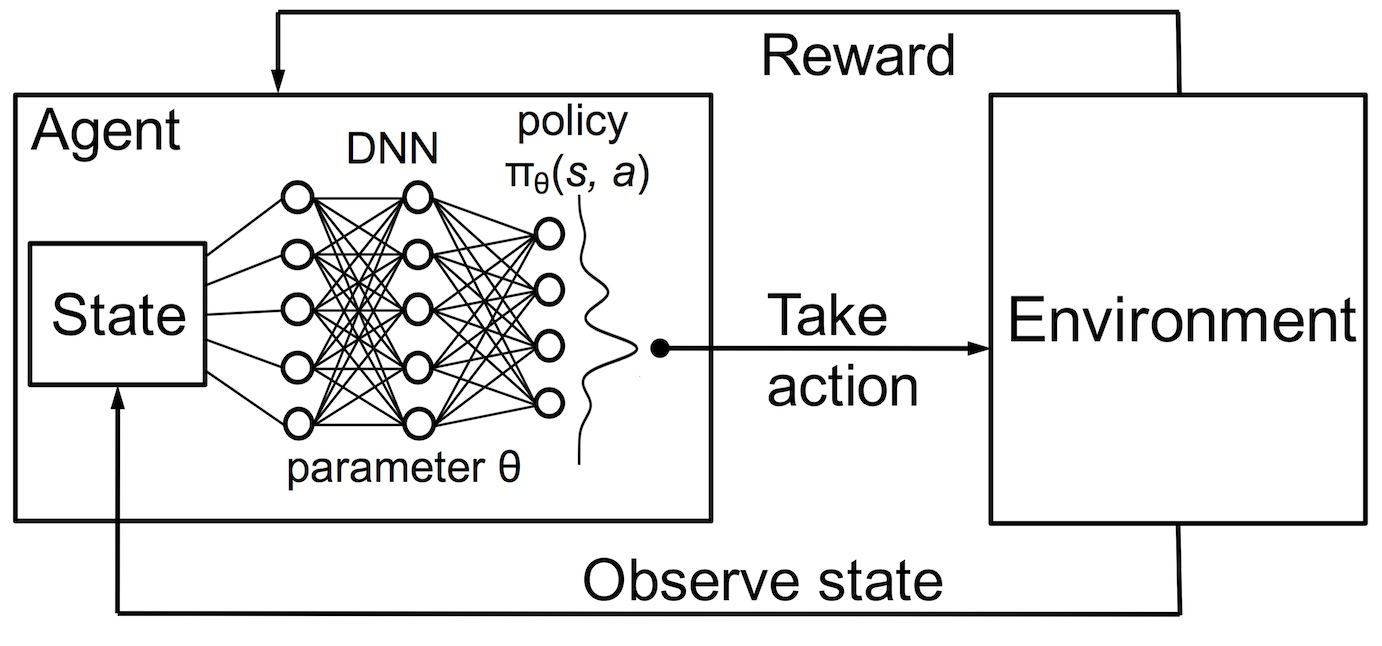
\includegraphics[width=0.5\textwidth]{chapters/chapter2/images/e2e-rl.jpg}
	\caption{Representation of end-to-end RL architctures
		\label{fig:e2e-rl}
	}
\end{figure}

As was mentioned in Section \ref{bg:sec:rl} there has been a renewed focus on the area of DRL. This research trend originated in 2013 when DeepMind showed that using a combination of Q-Learning and deep learning, it can produce agents that can compete with expert-humans in Atari.

\section{DQN on Atari 2600}
\label{bg:sec:dqn}
As mentioned in previous sections, one of the pioneering companies in the area was DeepMind. In 2013, V.Mnih et al. while working at DeepMind, released a paper titled \textit{``Playing Atari with Deep Reinforcement Learning''}\cite{dqn}. This paper combined DRL, convolutional neural networks and a novel strategy called \textbf{experience replay}. DeepMind, in 2014, patented Q-Learning and it's application with deep learning on Atari games. Further, they also published further papers expanding on the idea in prestigious journals such as NIPS and Nature. Figure \ref{fig:q-learning-arch} shows the structure of a Deep Q-Network as used to play Atari 2600 games.

Experience replay was an important improvement that helped in stabilising the Q-Learning algorithm. It does this by removing the correlations between a observation sequence, i.e. we don't learn from a chronological series of frames, rather we store all the experience and learn using random samples of this memory.

Over the following few years, this area would see rapid progress with many different advancements by both DeepMind and OpenAI. As was noted with the introduction of Deep Q-Learning (often referred to as `\textit{Deep Q-Networks}' or \textit{DQN}) the algorithm sufferes from overestimating the value of some actions. This can lead to a poor performance on more complex Atari games such as Space Invaders. Further detailed descriptions of the Q-Learning algorithm is provided in Section \ref{dsgn:sec:qlearning}.

\begin{figure}[htbp]
	\centering
	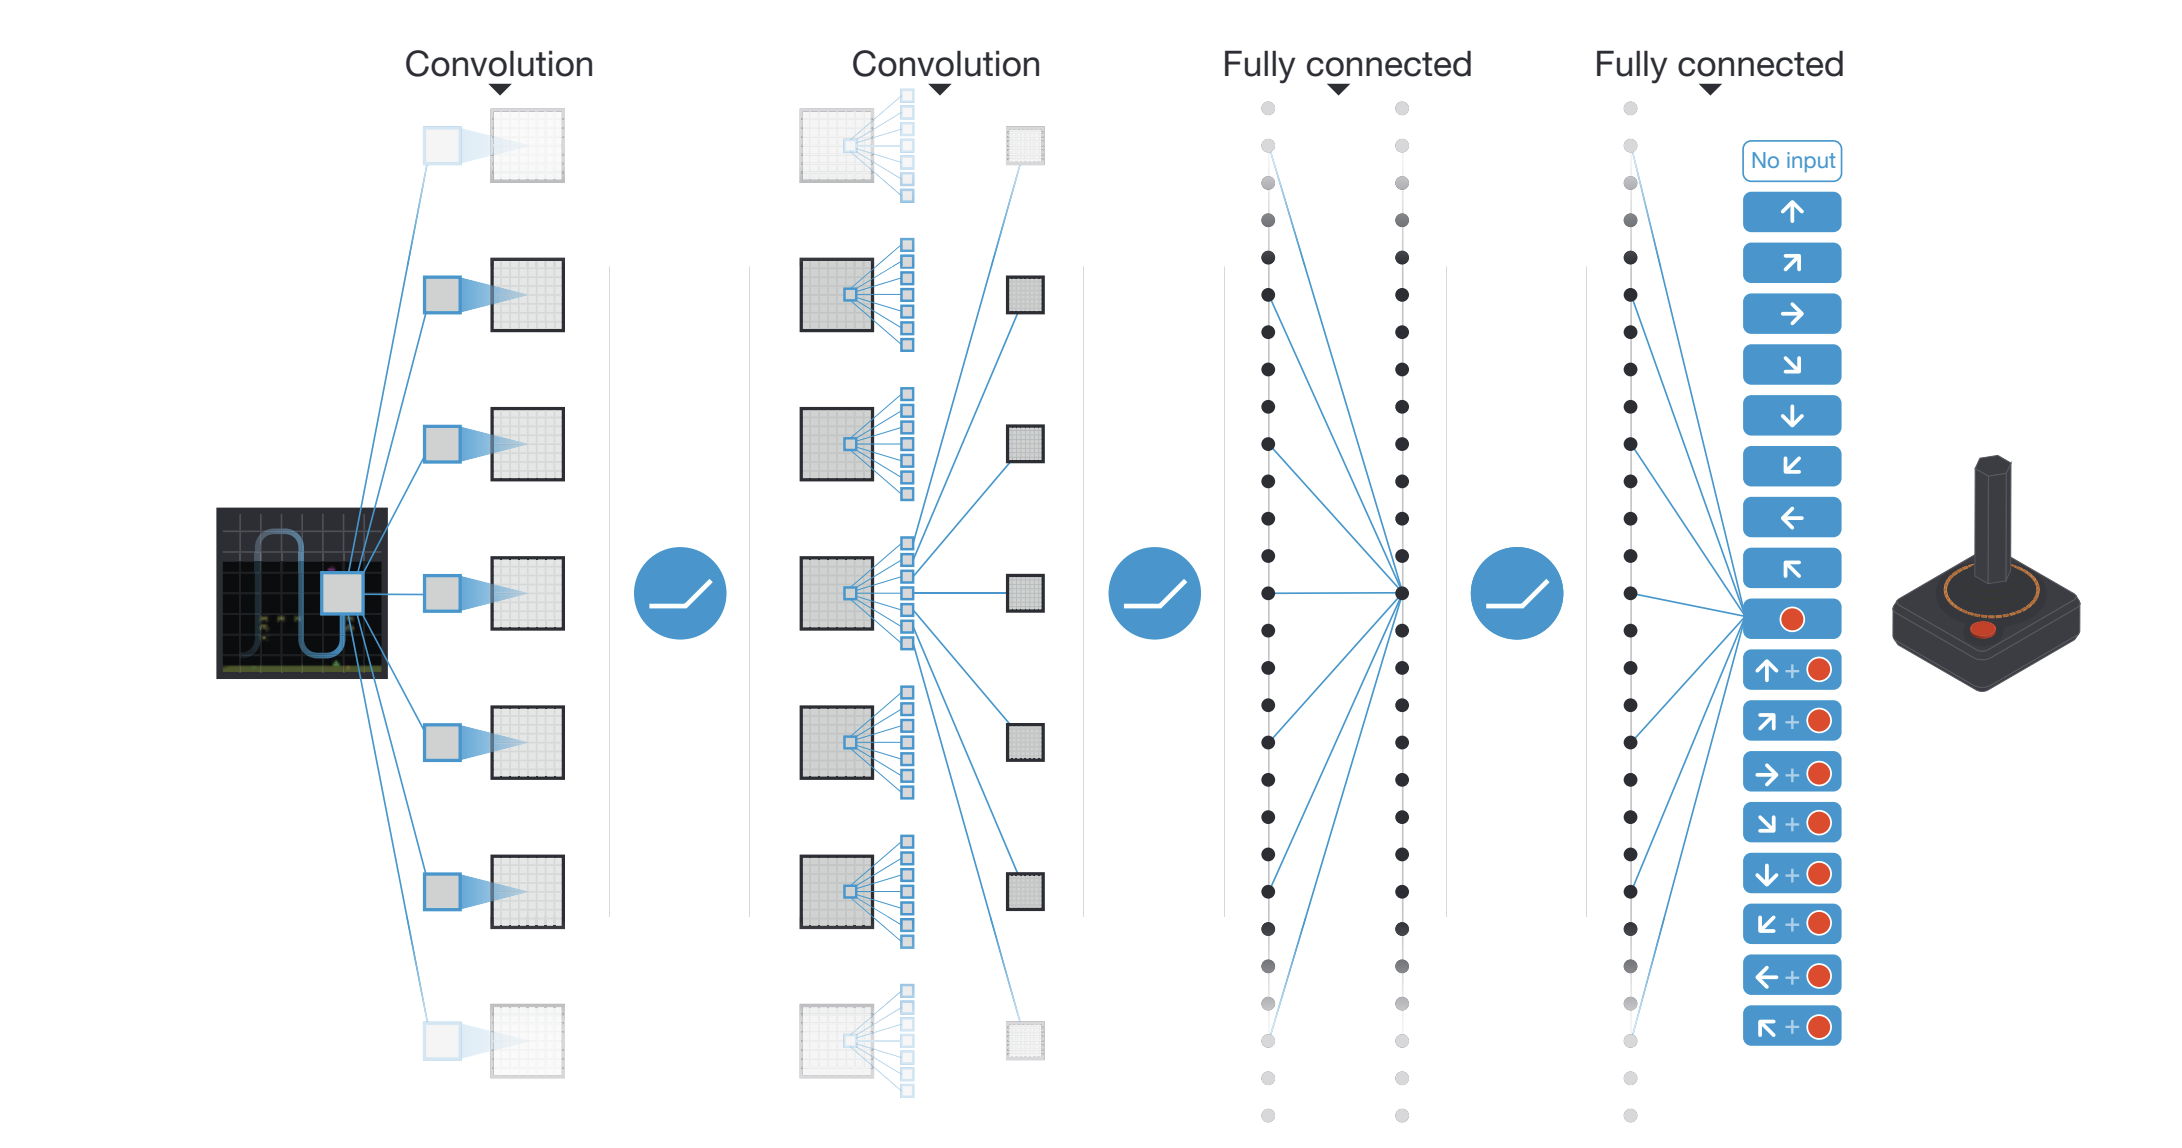
\includegraphics[width=0.75\textwidth]{chapters/chapter2/images/dqn.png}
	\caption[Deep Q-Network architcture]{Deep Q-Network architcture that from left-to-right is showing how a single frame is processed. First passing through convolutional layers, before being flattened to a single tensor which is connected to a fully connected network. This MLP acts as the Q-function approximator which will produce an output of predicted Q-values for each action.
		\label{fig:q-learning-arch}
	}
\end{figure}



\newpage

\section{CNN Visualisation}
\label{bg:sec:cnn-vis}
A common critisism of Neural Networks is that what the network learns is difficult to understand and interpret, therefore, over recent years some methods have been developed in order to visualise how the network learns. This section will describe some of the most common methods and those that produce the most visually pleasing results.

There are some considerations we need to make when visualising the CNN, for example, if we include a ReLU layer, the ReLU neurons don't have a semantic meaning by themselves. On the otherhand, in the individual filters in a CONV layer, we can observe the layer activations which indicate whether or not the network is converging.

\begin{figure}[ht!]
	\centering
	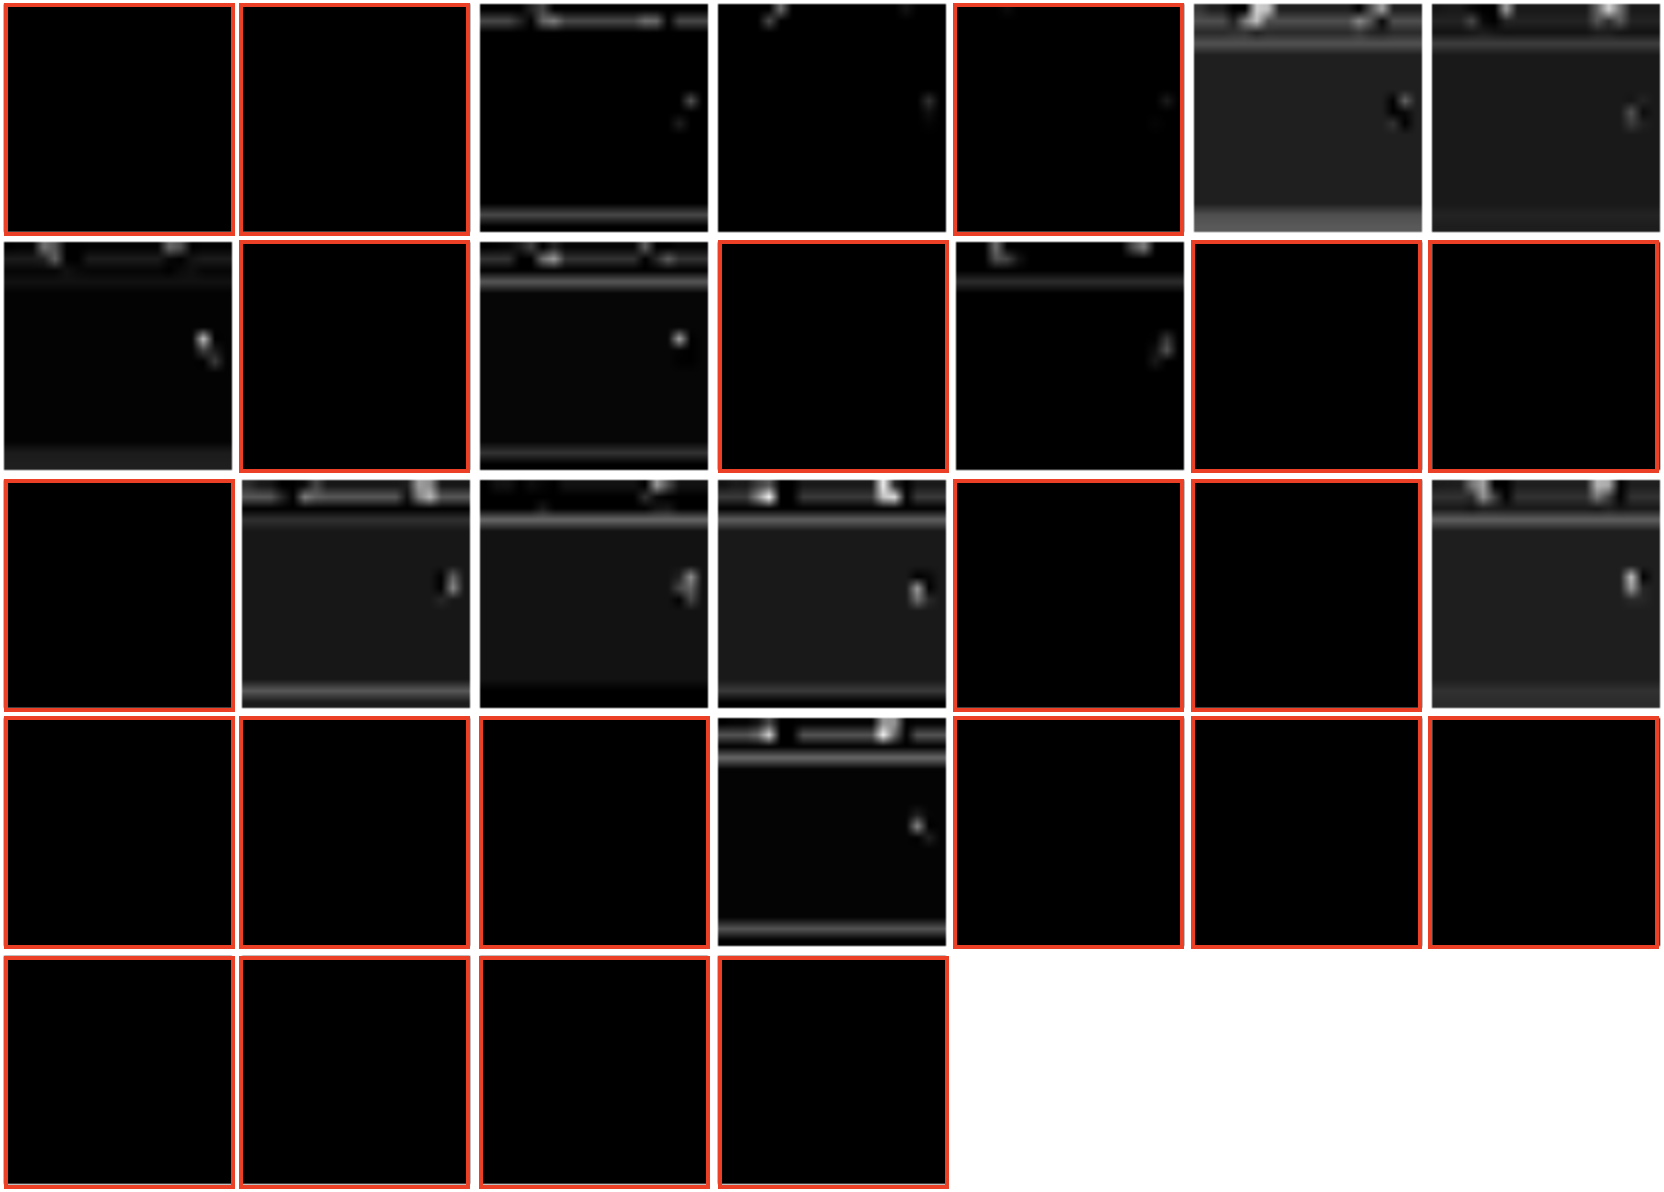
\includegraphics[width=0.75\textwidth]{chapters/chapter2/images/viz.png}
	\caption[Visualisation of the filters from the first layer of a CNN used to play Pong]{Visualisation of the first CONV layer of a CNN to play Pong, there are many filters completely black, in this agent, it means the learning rate was too high. Red highlighted filters are those filters with zero activation.
		\label{fig:cnn-viz-activ}
	}
\end{figure}

Based on Figure \ref{fig:cnn-viz-activ}, some of the filters show zero activation which can be a symptom of a high learning rate; these are often called \textit{``dead''} filters. Also, in terms of Atari games, during training, we can see what features the network is focusing on in attempt to maximise the rewards. Based on this information, one can tune both the learning rate during fine-tuning in order to extract more performance from the model.

In addition to visualising the individual layers of the CNN, there are some more advanced visualisation techniques. A common approach is to use Principle Component Analysis (PCA) which can be used to reduce the number of dimensions of the fully-connected layers down to 2 dimensions, showing the variance of each principal component which can allow the researcher to construct a new dataset that will improve the performance using the components with a high variance.

Another, more complex algorithm is called t-SNE  \cite{vanDerMaaten2008} which is a dimensionality reduction algorithm for high-dimensional datasets. It has been known to continuously produce visually pleasing results and was used in some of the papers referenced during the development of this project.
